\documentclass{beamer}
\usepackage[utf8]{inputenc}
\usepackage[]{amsmath}
\usepackage{graphicx}
\usepackage{physics}
\usepackage{subcaption} % package pour faire des subfigures
\usepackage{multirow} % package pour multirow/multicolumn
\usepackage{booktabs} % package pour top/mid/bottom rule
\usepackage{tcolorbox} % toujours plus de boites
%\usepackage[backend=biber]{biblatex}
%
%
%\addbibresource{Biblio_dbl_quantum.bib}

%\bibliographystyle{stylename}
%\bibliography{Biblio_dbl_quantum}

\title{Dipolar interactions in dense ensembles of Nitrogen-Vacancy centers}
\author{Clément Pellet-Mary, Maxime Perdriat, Gabriel Hétet}
\date{Nano-optics group}

\mode<presentation> {\usetheme{Rochester}}

\begin{document}
\begin{frame}
\maketitle
\begin{center}
\includegraphics[width=\textwidth,height=0.3\textheight,keepaspectratio]{logos}
\end{center}
\end{frame}
%\begin{frame}{Outline}
%\tableofcontents
%\end{frame}
%\section{Physics of the NV center}
\begin{frame}{Preamble : the NV center}
\centering
\includegraphics[width=\textwidth,height=0.9\textheight,keepaspectratio]{Slide  NV properties}
\end{frame}

\begin{frame}{Preamble : the 4 classes of NV centers}
\centering
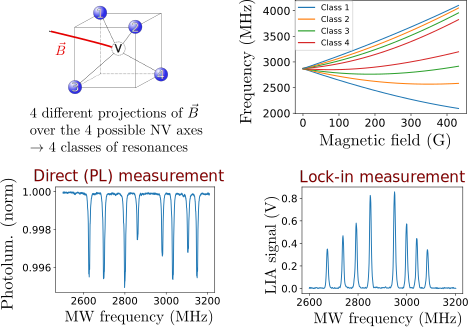
\includegraphics[width=\textwidth,height=0.9\textheight,keepaspectratio]{slide ODMR 4 classes}
\end{frame}

\begin{frame}{Depolarization of dense NV ensemble at low magnetic field}
\centering
\includegraphics[width=\textwidth,height=0.9\textheight,keepaspectratio]{slide_presentation_sujet}

\begin{frame}{outline}
\tableofcontents
\end{frame}

\section{Cross-relaxation with NV centers}
1 slide théorie CR + relation T1 PL
1 slide NV-VH
1 slide NV-NV : pb
\section{The NV-fluctuator model}

\section{Dipole-dipole interaction at low magnetic field}

\section{Charcterization of the low field depolarization magnetometry}


\end{frame}





\end{document}